
% Default to the notebook output style

    


% Inherit from the specified cell style.




    
\documentclass[11pt]{article}

    
    
    \usepackage[T1]{fontenc}
    % Nicer default font (+ math font) than Computer Modern for most use cases
    \usepackage{mathpazo}

    % Basic figure setup, for now with no caption control since it's done
    % automatically by Pandoc (which extracts ![](path) syntax from Markdown).
    \usepackage{graphicx}
    % We will generate all images so they have a width \maxwidth. This means
    % that they will get their normal width if they fit onto the page, but
    % are scaled down if they would overflow the margins.
    \makeatletter
    \def\maxwidth{\ifdim\Gin@nat@width>\linewidth\linewidth
    \else\Gin@nat@width\fi}
    \makeatother
    \let\Oldincludegraphics\includegraphics
    % Set max figure width to be 80% of text width, for now hardcoded.
    \renewcommand{\includegraphics}[1]{\Oldincludegraphics[width=.8\maxwidth]{#1}}
    % Ensure that by default, figures have no caption (until we provide a
    % proper Figure object with a Caption API and a way to capture that
    % in the conversion process - todo).
    \usepackage{caption}
    \DeclareCaptionLabelFormat{nolabel}{}
    \captionsetup{labelformat=nolabel}

    \usepackage{adjustbox} % Used to constrain images to a maximum size 
    \usepackage{xcolor} % Allow colors to be defined
    \usepackage{enumerate} % Needed for markdown enumerations to work
    \usepackage{geometry} % Used to adjust the document margins
    \usepackage{amsmath} % Equations
    \usepackage{amssymb} % Equations
    \usepackage{textcomp} % defines textquotesingle
    % Hack from http://tex.stackexchange.com/a/47451/13684:
    \AtBeginDocument{%
        \def\PYZsq{\textquotesingle}% Upright quotes in Pygmentized code
    }
    \usepackage{upquote} % Upright quotes for verbatim code
    \usepackage{eurosym} % defines \euro
    \usepackage[mathletters]{ucs} % Extended unicode (utf-8) support
    \usepackage[utf8x]{inputenc} % Allow utf-8 characters in the tex document
    \usepackage{fancyvrb} % verbatim replacement that allows latex
    \usepackage{grffile} % extends the file name processing of package graphics 
                         % to support a larger range 
    % The hyperref package gives us a pdf with properly built
    % internal navigation ('pdf bookmarks' for the table of contents,
    % internal cross-reference links, web links for URLs, etc.)
    \usepackage{hyperref}
    \usepackage{longtable} % longtable support required by pandoc >1.10
    \usepackage{booktabs}  % table support for pandoc > 1.12.2
    \usepackage[inline]{enumitem} % IRkernel/repr support (it uses the enumerate* environment)
    \usepackage[normalem]{ulem} % ulem is needed to support strikethroughs (\sout)
                                % normalem makes italics be italics, not underlines
    

    
    
    % Colors for the hyperref package
    \definecolor{urlcolor}{rgb}{0,.145,.698}
    \definecolor{linkcolor}{rgb}{.71,0.21,0.01}
    \definecolor{citecolor}{rgb}{.12,.54,.11}

    % ANSI colors
    \definecolor{ansi-black}{HTML}{3E424D}
    \definecolor{ansi-black-intense}{HTML}{282C36}
    \definecolor{ansi-red}{HTML}{E75C58}
    \definecolor{ansi-red-intense}{HTML}{B22B31}
    \definecolor{ansi-green}{HTML}{00A250}
    \definecolor{ansi-green-intense}{HTML}{007427}
    \definecolor{ansi-yellow}{HTML}{DDB62B}
    \definecolor{ansi-yellow-intense}{HTML}{B27D12}
    \definecolor{ansi-blue}{HTML}{208FFB}
    \definecolor{ansi-blue-intense}{HTML}{0065CA}
    \definecolor{ansi-magenta}{HTML}{D160C4}
    \definecolor{ansi-magenta-intense}{HTML}{A03196}
    \definecolor{ansi-cyan}{HTML}{60C6C8}
    \definecolor{ansi-cyan-intense}{HTML}{258F8F}
    \definecolor{ansi-white}{HTML}{C5C1B4}
    \definecolor{ansi-white-intense}{HTML}{A1A6B2}

    % commands and environments needed by pandoc snippets
    % extracted from the output of `pandoc -s`
    \providecommand{\tightlist}{%
      \setlength{\itemsep}{0pt}\setlength{\parskip}{0pt}}
    \DefineVerbatimEnvironment{Highlighting}{Verbatim}{commandchars=\\\{\}}
    % Add ',fontsize=\small' for more characters per line
    \newenvironment{Shaded}{}{}
    \newcommand{\KeywordTok}[1]{\textcolor[rgb]{0.00,0.44,0.13}{\textbf{{#1}}}}
    \newcommand{\DataTypeTok}[1]{\textcolor[rgb]{0.56,0.13,0.00}{{#1}}}
    \newcommand{\DecValTok}[1]{\textcolor[rgb]{0.25,0.63,0.44}{{#1}}}
    \newcommand{\BaseNTok}[1]{\textcolor[rgb]{0.25,0.63,0.44}{{#1}}}
    \newcommand{\FloatTok}[1]{\textcolor[rgb]{0.25,0.63,0.44}{{#1}}}
    \newcommand{\CharTok}[1]{\textcolor[rgb]{0.25,0.44,0.63}{{#1}}}
    \newcommand{\StringTok}[1]{\textcolor[rgb]{0.25,0.44,0.63}{{#1}}}
    \newcommand{\CommentTok}[1]{\textcolor[rgb]{0.38,0.63,0.69}{\textit{{#1}}}}
    \newcommand{\OtherTok}[1]{\textcolor[rgb]{0.00,0.44,0.13}{{#1}}}
    \newcommand{\AlertTok}[1]{\textcolor[rgb]{1.00,0.00,0.00}{\textbf{{#1}}}}
    \newcommand{\FunctionTok}[1]{\textcolor[rgb]{0.02,0.16,0.49}{{#1}}}
    \newcommand{\RegionMarkerTok}[1]{{#1}}
    \newcommand{\ErrorTok}[1]{\textcolor[rgb]{1.00,0.00,0.00}{\textbf{{#1}}}}
    \newcommand{\NormalTok}[1]{{#1}}
    
    % Additional commands for more recent versions of Pandoc
    \newcommand{\ConstantTok}[1]{\textcolor[rgb]{0.53,0.00,0.00}{{#1}}}
    \newcommand{\SpecialCharTok}[1]{\textcolor[rgb]{0.25,0.44,0.63}{{#1}}}
    \newcommand{\VerbatimStringTok}[1]{\textcolor[rgb]{0.25,0.44,0.63}{{#1}}}
    \newcommand{\SpecialStringTok}[1]{\textcolor[rgb]{0.73,0.40,0.53}{{#1}}}
    \newcommand{\ImportTok}[1]{{#1}}
    \newcommand{\DocumentationTok}[1]{\textcolor[rgb]{0.73,0.13,0.13}{\textit{{#1}}}}
    \newcommand{\AnnotationTok}[1]{\textcolor[rgb]{0.38,0.63,0.69}{\textbf{\textit{{#1}}}}}
    \newcommand{\CommentVarTok}[1]{\textcolor[rgb]{0.38,0.63,0.69}{\textbf{\textit{{#1}}}}}
    \newcommand{\VariableTok}[1]{\textcolor[rgb]{0.10,0.09,0.49}{{#1}}}
    \newcommand{\ControlFlowTok}[1]{\textcolor[rgb]{0.00,0.44,0.13}{\textbf{{#1}}}}
    \newcommand{\OperatorTok}[1]{\textcolor[rgb]{0.40,0.40,0.40}{{#1}}}
    \newcommand{\BuiltInTok}[1]{{#1}}
    \newcommand{\ExtensionTok}[1]{{#1}}
    \newcommand{\PreprocessorTok}[1]{\textcolor[rgb]{0.74,0.48,0.00}{{#1}}}
    \newcommand{\AttributeTok}[1]{\textcolor[rgb]{0.49,0.56,0.16}{{#1}}}
    \newcommand{\InformationTok}[1]{\textcolor[rgb]{0.38,0.63,0.69}{\textbf{\textit{{#1}}}}}
    \newcommand{\WarningTok}[1]{\textcolor[rgb]{0.38,0.63,0.69}{\textbf{\textit{{#1}}}}}
    
    
    % Define a nice break command that doesn't care if a line doesn't already
    % exist.
    \def\br{\hspace*{\fill} \\* }
    % Math Jax compatability definitions
    \def\gt{>}
    \def\lt{<}
    % Document parameters
    \title{TP\_Junier}
    
    
    

    % Pygments definitions
    
\makeatletter
\def\PY@reset{\let\PY@it=\relax \let\PY@bf=\relax%
    \let\PY@ul=\relax \let\PY@tc=\relax%
    \let\PY@bc=\relax \let\PY@ff=\relax}
\def\PY@tok#1{\csname PY@tok@#1\endcsname}
\def\PY@toks#1+{\ifx\relax#1\empty\else%
    \PY@tok{#1}\expandafter\PY@toks\fi}
\def\PY@do#1{\PY@bc{\PY@tc{\PY@ul{%
    \PY@it{\PY@bf{\PY@ff{#1}}}}}}}
\def\PY#1#2{\PY@reset\PY@toks#1+\relax+\PY@do{#2}}

\expandafter\def\csname PY@tok@w\endcsname{\def\PY@tc##1{\textcolor[rgb]{0.73,0.73,0.73}{##1}}}
\expandafter\def\csname PY@tok@c\endcsname{\let\PY@it=\textit\def\PY@tc##1{\textcolor[rgb]{0.25,0.50,0.50}{##1}}}
\expandafter\def\csname PY@tok@cp\endcsname{\def\PY@tc##1{\textcolor[rgb]{0.74,0.48,0.00}{##1}}}
\expandafter\def\csname PY@tok@k\endcsname{\let\PY@bf=\textbf\def\PY@tc##1{\textcolor[rgb]{0.00,0.50,0.00}{##1}}}
\expandafter\def\csname PY@tok@kp\endcsname{\def\PY@tc##1{\textcolor[rgb]{0.00,0.50,0.00}{##1}}}
\expandafter\def\csname PY@tok@kt\endcsname{\def\PY@tc##1{\textcolor[rgb]{0.69,0.00,0.25}{##1}}}
\expandafter\def\csname PY@tok@o\endcsname{\def\PY@tc##1{\textcolor[rgb]{0.40,0.40,0.40}{##1}}}
\expandafter\def\csname PY@tok@ow\endcsname{\let\PY@bf=\textbf\def\PY@tc##1{\textcolor[rgb]{0.67,0.13,1.00}{##1}}}
\expandafter\def\csname PY@tok@nb\endcsname{\def\PY@tc##1{\textcolor[rgb]{0.00,0.50,0.00}{##1}}}
\expandafter\def\csname PY@tok@nf\endcsname{\def\PY@tc##1{\textcolor[rgb]{0.00,0.00,1.00}{##1}}}
\expandafter\def\csname PY@tok@nc\endcsname{\let\PY@bf=\textbf\def\PY@tc##1{\textcolor[rgb]{0.00,0.00,1.00}{##1}}}
\expandafter\def\csname PY@tok@nn\endcsname{\let\PY@bf=\textbf\def\PY@tc##1{\textcolor[rgb]{0.00,0.00,1.00}{##1}}}
\expandafter\def\csname PY@tok@ne\endcsname{\let\PY@bf=\textbf\def\PY@tc##1{\textcolor[rgb]{0.82,0.25,0.23}{##1}}}
\expandafter\def\csname PY@tok@nv\endcsname{\def\PY@tc##1{\textcolor[rgb]{0.10,0.09,0.49}{##1}}}
\expandafter\def\csname PY@tok@no\endcsname{\def\PY@tc##1{\textcolor[rgb]{0.53,0.00,0.00}{##1}}}
\expandafter\def\csname PY@tok@nl\endcsname{\def\PY@tc##1{\textcolor[rgb]{0.63,0.63,0.00}{##1}}}
\expandafter\def\csname PY@tok@ni\endcsname{\let\PY@bf=\textbf\def\PY@tc##1{\textcolor[rgb]{0.60,0.60,0.60}{##1}}}
\expandafter\def\csname PY@tok@na\endcsname{\def\PY@tc##1{\textcolor[rgb]{0.49,0.56,0.16}{##1}}}
\expandafter\def\csname PY@tok@nt\endcsname{\let\PY@bf=\textbf\def\PY@tc##1{\textcolor[rgb]{0.00,0.50,0.00}{##1}}}
\expandafter\def\csname PY@tok@nd\endcsname{\def\PY@tc##1{\textcolor[rgb]{0.67,0.13,1.00}{##1}}}
\expandafter\def\csname PY@tok@s\endcsname{\def\PY@tc##1{\textcolor[rgb]{0.73,0.13,0.13}{##1}}}
\expandafter\def\csname PY@tok@sd\endcsname{\let\PY@it=\textit\def\PY@tc##1{\textcolor[rgb]{0.73,0.13,0.13}{##1}}}
\expandafter\def\csname PY@tok@si\endcsname{\let\PY@bf=\textbf\def\PY@tc##1{\textcolor[rgb]{0.73,0.40,0.53}{##1}}}
\expandafter\def\csname PY@tok@se\endcsname{\let\PY@bf=\textbf\def\PY@tc##1{\textcolor[rgb]{0.73,0.40,0.13}{##1}}}
\expandafter\def\csname PY@tok@sr\endcsname{\def\PY@tc##1{\textcolor[rgb]{0.73,0.40,0.53}{##1}}}
\expandafter\def\csname PY@tok@ss\endcsname{\def\PY@tc##1{\textcolor[rgb]{0.10,0.09,0.49}{##1}}}
\expandafter\def\csname PY@tok@sx\endcsname{\def\PY@tc##1{\textcolor[rgb]{0.00,0.50,0.00}{##1}}}
\expandafter\def\csname PY@tok@m\endcsname{\def\PY@tc##1{\textcolor[rgb]{0.40,0.40,0.40}{##1}}}
\expandafter\def\csname PY@tok@gh\endcsname{\let\PY@bf=\textbf\def\PY@tc##1{\textcolor[rgb]{0.00,0.00,0.50}{##1}}}
\expandafter\def\csname PY@tok@gu\endcsname{\let\PY@bf=\textbf\def\PY@tc##1{\textcolor[rgb]{0.50,0.00,0.50}{##1}}}
\expandafter\def\csname PY@tok@gd\endcsname{\def\PY@tc##1{\textcolor[rgb]{0.63,0.00,0.00}{##1}}}
\expandafter\def\csname PY@tok@gi\endcsname{\def\PY@tc##1{\textcolor[rgb]{0.00,0.63,0.00}{##1}}}
\expandafter\def\csname PY@tok@gr\endcsname{\def\PY@tc##1{\textcolor[rgb]{1.00,0.00,0.00}{##1}}}
\expandafter\def\csname PY@tok@ge\endcsname{\let\PY@it=\textit}
\expandafter\def\csname PY@tok@gs\endcsname{\let\PY@bf=\textbf}
\expandafter\def\csname PY@tok@gp\endcsname{\let\PY@bf=\textbf\def\PY@tc##1{\textcolor[rgb]{0.00,0.00,0.50}{##1}}}
\expandafter\def\csname PY@tok@go\endcsname{\def\PY@tc##1{\textcolor[rgb]{0.53,0.53,0.53}{##1}}}
\expandafter\def\csname PY@tok@gt\endcsname{\def\PY@tc##1{\textcolor[rgb]{0.00,0.27,0.87}{##1}}}
\expandafter\def\csname PY@tok@err\endcsname{\def\PY@bc##1{\setlength{\fboxsep}{0pt}\fcolorbox[rgb]{1.00,0.00,0.00}{1,1,1}{\strut ##1}}}
\expandafter\def\csname PY@tok@kc\endcsname{\let\PY@bf=\textbf\def\PY@tc##1{\textcolor[rgb]{0.00,0.50,0.00}{##1}}}
\expandafter\def\csname PY@tok@kd\endcsname{\let\PY@bf=\textbf\def\PY@tc##1{\textcolor[rgb]{0.00,0.50,0.00}{##1}}}
\expandafter\def\csname PY@tok@kn\endcsname{\let\PY@bf=\textbf\def\PY@tc##1{\textcolor[rgb]{0.00,0.50,0.00}{##1}}}
\expandafter\def\csname PY@tok@kr\endcsname{\let\PY@bf=\textbf\def\PY@tc##1{\textcolor[rgb]{0.00,0.50,0.00}{##1}}}
\expandafter\def\csname PY@tok@bp\endcsname{\def\PY@tc##1{\textcolor[rgb]{0.00,0.50,0.00}{##1}}}
\expandafter\def\csname PY@tok@fm\endcsname{\def\PY@tc##1{\textcolor[rgb]{0.00,0.00,1.00}{##1}}}
\expandafter\def\csname PY@tok@vc\endcsname{\def\PY@tc##1{\textcolor[rgb]{0.10,0.09,0.49}{##1}}}
\expandafter\def\csname PY@tok@vg\endcsname{\def\PY@tc##1{\textcolor[rgb]{0.10,0.09,0.49}{##1}}}
\expandafter\def\csname PY@tok@vi\endcsname{\def\PY@tc##1{\textcolor[rgb]{0.10,0.09,0.49}{##1}}}
\expandafter\def\csname PY@tok@vm\endcsname{\def\PY@tc##1{\textcolor[rgb]{0.10,0.09,0.49}{##1}}}
\expandafter\def\csname PY@tok@sa\endcsname{\def\PY@tc##1{\textcolor[rgb]{0.73,0.13,0.13}{##1}}}
\expandafter\def\csname PY@tok@sb\endcsname{\def\PY@tc##1{\textcolor[rgb]{0.73,0.13,0.13}{##1}}}
\expandafter\def\csname PY@tok@sc\endcsname{\def\PY@tc##1{\textcolor[rgb]{0.73,0.13,0.13}{##1}}}
\expandafter\def\csname PY@tok@dl\endcsname{\def\PY@tc##1{\textcolor[rgb]{0.73,0.13,0.13}{##1}}}
\expandafter\def\csname PY@tok@s2\endcsname{\def\PY@tc##1{\textcolor[rgb]{0.73,0.13,0.13}{##1}}}
\expandafter\def\csname PY@tok@sh\endcsname{\def\PY@tc##1{\textcolor[rgb]{0.73,0.13,0.13}{##1}}}
\expandafter\def\csname PY@tok@s1\endcsname{\def\PY@tc##1{\textcolor[rgb]{0.73,0.13,0.13}{##1}}}
\expandafter\def\csname PY@tok@mb\endcsname{\def\PY@tc##1{\textcolor[rgb]{0.40,0.40,0.40}{##1}}}
\expandafter\def\csname PY@tok@mf\endcsname{\def\PY@tc##1{\textcolor[rgb]{0.40,0.40,0.40}{##1}}}
\expandafter\def\csname PY@tok@mh\endcsname{\def\PY@tc##1{\textcolor[rgb]{0.40,0.40,0.40}{##1}}}
\expandafter\def\csname PY@tok@mi\endcsname{\def\PY@tc##1{\textcolor[rgb]{0.40,0.40,0.40}{##1}}}
\expandafter\def\csname PY@tok@il\endcsname{\def\PY@tc##1{\textcolor[rgb]{0.40,0.40,0.40}{##1}}}
\expandafter\def\csname PY@tok@mo\endcsname{\def\PY@tc##1{\textcolor[rgb]{0.40,0.40,0.40}{##1}}}
\expandafter\def\csname PY@tok@ch\endcsname{\let\PY@it=\textit\def\PY@tc##1{\textcolor[rgb]{0.25,0.50,0.50}{##1}}}
\expandafter\def\csname PY@tok@cm\endcsname{\let\PY@it=\textit\def\PY@tc##1{\textcolor[rgb]{0.25,0.50,0.50}{##1}}}
\expandafter\def\csname PY@tok@cpf\endcsname{\let\PY@it=\textit\def\PY@tc##1{\textcolor[rgb]{0.25,0.50,0.50}{##1}}}
\expandafter\def\csname PY@tok@c1\endcsname{\let\PY@it=\textit\def\PY@tc##1{\textcolor[rgb]{0.25,0.50,0.50}{##1}}}
\expandafter\def\csname PY@tok@cs\endcsname{\let\PY@it=\textit\def\PY@tc##1{\textcolor[rgb]{0.25,0.50,0.50}{##1}}}

\def\PYZbs{\char`\\}
\def\PYZus{\char`\_}
\def\PYZob{\char`\{}
\def\PYZcb{\char`\}}
\def\PYZca{\char`\^}
\def\PYZam{\char`\&}
\def\PYZlt{\char`\<}
\def\PYZgt{\char`\>}
\def\PYZsh{\char`\#}
\def\PYZpc{\char`\%}
\def\PYZdl{\char`\$}
\def\PYZhy{\char`\-}
\def\PYZsq{\char`\'}
\def\PYZdq{\char`\"}
\def\PYZti{\char`\~}
% for compatibility with earlier versions
\def\PYZat{@}
\def\PYZlb{[}
\def\PYZrb{]}
\makeatother


    % Exact colors from NB
    \definecolor{incolor}{rgb}{0.0, 0.0, 0.5}
    \definecolor{outcolor}{rgb}{0.545, 0.0, 0.0}



    
    % Prevent overflowing lines due to hard-to-break entities
    \sloppy 
    % Setup hyperref package
    \hypersetup{
      breaklinks=true,  % so long urls are correctly broken across lines
      colorlinks=true,
      urlcolor=urlcolor,
      linkcolor=linkcolor,
      citecolor=citecolor,
      }
    % Slightly bigger margins than the latex defaults
    
    \geometry{verbose,tmargin=1in,bmargin=1in,lmargin=1in,rmargin=1in}
    
    

    \begin{document}
    
    
    \maketitle
    
    

    
    \begin{Verbatim}[commandchars=\\\{\}]
{\color{incolor}In [{\color{incolor}2}]:} \PY{o}{\PYZpc{}}\PY{k}{reload\PYZus{}ext} sql
        \PY{o}{\PYZpc{}}\PY{k}{config} SqlMagic.displaycon = False
        \PY{o}{\PYZpc{}}\PY{k}{config} SqlMagic.autolimit = 100
\end{Verbatim}


    \begin{Verbatim}[commandchars=\\\{\}]
{\color{incolor}In [{\color{incolor}3}]:} \PY{o}{\PYZpc{}}\PY{k}{sql} sqlite:///base\PYZhy{}etudiant.db
\end{Verbatim}


    \hypertarget{exercice-1}{%
\section{Exercice 1:}\label{exercice-1}}

Donner tous les noms des étudiants.

    \begin{Verbatim}[commandchars=\\\{\}]
{\color{incolor}In [{\color{incolor}18}]:} \PY{o}{\PYZpc{}\PYZpc{}}\PY{k}{sql}
         
         SELECT NomEt FROM Etudiant;
\end{Verbatim}


    \begin{Verbatim}[commandchars=\\\{\}]
Done.

    \end{Verbatim}

\begin{Verbatim}[commandchars=\\\{\}]
{\color{outcolor}Out[{\color{outcolor}18}]:} [('Armand A.',),
          ('Berthe B.',),
          ('Cendrine C.',),
          ('David D.',),
          ('Erwan E.',),
          ('Fabien F.',),
          ('Gerald G.',),
          ('Herbert H.',),
          ('Jacques J.',)]
\end{Verbatim}
            
    \begin{Verbatim}[commandchars=\\\{\}]
{\color{incolor}In [{\color{incolor}17}]:} \PY{o}{\PYZpc{}\PYZpc{}}\PY{k}{sql} 
         SELECT *
         FROM sqlite\PYZus{}master
\end{Verbatim}


    \begin{Verbatim}[commandchars=\\\{\}]
Done.

    \end{Verbatim}

\begin{Verbatim}[commandchars=\\\{\}]
{\color{outcolor}Out[{\color{outcolor}17}]:} [('table', 'Etudiant', 'Etudiant', 2, 'CREATE TABLE Etudiant (\textbackslash{}n       NumEt INTEGER PRIMARY KEY,\textbackslash{}n       NomEt VARCHAR2(255),\textbackslash{}n       Adresse VARCHAR2(1000)\textbackslash{}n)'),
          ('table', 'Enseignant', 'Enseignant', 3, 'CREATE TABLE Enseignant (\textbackslash{}n       NumEns INTEGER PRIMARY KEY,\textbackslash{}n       NomEns VARCHAR2(255)\textbackslash{}n)'),
          ('table', 'UE', 'UE', 4, 'CREATE TABLE UE (\textbackslash{}n       NumUE INTEGER PRIMARY KEY,\textbackslash{}n       Titre VARCHAR2(255),\textbackslash{}n       HCours FLOAT,\textbackslash{}n       HTD FLOAT,\textbackslash{}n       HTP FLOAT\textbackslash{}n)'),
          ('table', 'Enseigne', 'Enseigne', 5, 'CREATE TABLE Enseigne (\textbackslash{}n       NumEns INTEGER REFERENCES Enseignant(NumEns),\textbackslash{}n       NumUE INTEGER REFERENCES UE(NumUE),\textbackslash{}n       NCours INTEGER,\textbackslash{}n       NTD INTEGER,\textbackslash{}n       NTP INTEGER,\textbackslash{}n       PRIMARY KEY (NumEns,NumUE)\textbackslash{}n)'),
          ('index', 'sqlite\_autoindex\_Enseigne\_1', 'Enseigne', 6, None),
          ('table', 'Inscrit', 'Inscrit', 7, 'CREATE TABLE Inscrit (\textbackslash{}n       NumEt INTEGER REFERENCES Etudiant(NumEt),\textbackslash{}n       NumUE INTEGER REFERENCES UE(NumUE),\textbackslash{}n       PRIMARY KEY (NumEt,NumUE)\textbackslash{}n)'),
          ('index', 'sqlite\_autoindex\_Inscrit\_1', 'Inscrit', 8, None)]
\end{Verbatim}
            
    \begin{Verbatim}[commandchars=\\\{\}]
{\color{incolor}In [{\color{incolor}6}]:} \PY{o}{\PYZpc{}\PYZpc{}}\PY{k}{sql}
        
        SELECT name 
        FROM sqlite\PYZus{}master
        WHERE type = \PYZsq{}table\PYZsq{}
\end{Verbatim}


    \begin{Verbatim}[commandchars=\\\{\}]
Done.

    \end{Verbatim}

\begin{Verbatim}[commandchars=\\\{\}]
{\color{outcolor}Out[{\color{outcolor}6}]:} [('Etudiant',), ('Enseignant',), ('UE',), ('Enseigne',), ('Inscrit',)]
\end{Verbatim}
            
    \begin{Verbatim}[commandchars=\\\{\}]
{\color{incolor}In [{\color{incolor}13}]:} \PY{o}{\PYZpc{}\PYZpc{}}\PY{k}{sql}
         
         SELECT sql 
         FROM sqlite\PYZus{}master
         WHERE name = \PYZsq{}Etudiant\PYZsq{};
\end{Verbatim}


    \begin{Verbatim}[commandchars=\\\{\}]
Done.

    \end{Verbatim}

\begin{Verbatim}[commandchars=\\\{\}]
{\color{outcolor}Out[{\color{outcolor}13}]:} [('CREATE TABLE Etudiant (\textbackslash{}n       NumEt INTEGER PRIMARY KEY,\textbackslash{}n       NomEt VARCHAR2(255),\textbackslash{}n       Adresse VARCHAR2(1000)\textbackslash{}n)',)]
\end{Verbatim}
            
    \begin{Verbatim}[commandchars=\\\{\}]
{\color{incolor}In [{\color{incolor}9}]:} \PY{o}{\PYZpc{}\PYZpc{}}\PY{k}{sql}
        
        SELECT sql 
        FROM sqlite\PYZus{}master
        WHERE name = \PYZsq{}Enseignant\PYZsq{};
\end{Verbatim}


    \begin{Verbatim}[commandchars=\\\{\}]
Done.

    \end{Verbatim}

\begin{Verbatim}[commandchars=\\\{\}]
{\color{outcolor}Out[{\color{outcolor}9}]:} [('CREATE TABLE Enseignant (\textbackslash{}n       NumEns INTEGER PRIMARY KEY,\textbackslash{}n       NomEns VARCHAR2(255)\textbackslash{}n)',)]
\end{Verbatim}
            
    \begin{Verbatim}[commandchars=\\\{\}]
{\color{incolor}In [{\color{incolor}14}]:} \PY{o}{\PYZpc{}\PYZpc{}}\PY{k}{sql}
         
         SELECT sql 
         FROM sqlite\PYZus{}master
         WHERE name = \PYZsq{}UE\PYZsq{};
\end{Verbatim}


    \begin{Verbatim}[commandchars=\\\{\}]
Done.

    \end{Verbatim}

\begin{Verbatim}[commandchars=\\\{\}]
{\color{outcolor}Out[{\color{outcolor}14}]:} [('CREATE TABLE UE (\textbackslash{}n       NumUE INTEGER PRIMARY KEY,\textbackslash{}n       Titre VARCHAR2(255),\textbackslash{}n       HCours FLOAT,\textbackslash{}n       HTD FLOAT,\textbackslash{}n       HTP FLOAT\textbackslash{}n)',)]
\end{Verbatim}
            
    \begin{Verbatim}[commandchars=\\\{\}]
{\color{incolor}In [{\color{incolor}15}]:} \PY{o}{\PYZpc{}\PYZpc{}}\PY{k}{sql}
         
         SELECT sql 
         FROM sqlite\PYZus{}master
         WHERE name = \PYZsq{}Enseigne\PYZsq{};
\end{Verbatim}


    \begin{Verbatim}[commandchars=\\\{\}]
Done.

    \end{Verbatim}

\begin{Verbatim}[commandchars=\\\{\}]
{\color{outcolor}Out[{\color{outcolor}15}]:} [('CREATE TABLE Enseigne (\textbackslash{}n       NumEns INTEGER REFERENCES Enseignant(NumEns),\textbackslash{}n       NumUE INTEGER REFERENCES UE(NumUE),\textbackslash{}n       NCours INTEGER,\textbackslash{}n       NTD INTEGER,\textbackslash{}n       NTP INTEGER,\textbackslash{}n       PRIMARY KEY (NumEns,NumUE)\textbackslash{}n)',)]
\end{Verbatim}
            
    \begin{Verbatim}[commandchars=\\\{\}]
{\color{incolor}In [{\color{incolor}16}]:} \PY{o}{\PYZpc{}\PYZpc{}}\PY{k}{sql}
         
         SELECT sql 
         FROM sqlite\PYZus{}master
         WHERE name = \PYZsq{}Inscrit\PYZsq{};
\end{Verbatim}


    \begin{Verbatim}[commandchars=\\\{\}]
Done.

    \end{Verbatim}

\begin{Verbatim}[commandchars=\\\{\}]
{\color{outcolor}Out[{\color{outcolor}16}]:} [('CREATE TABLE Inscrit (\textbackslash{}n       NumEt INTEGER REFERENCES Etudiant(NumEt),\textbackslash{}n       NumUE INTEGER REFERENCES UE(NumUE),\textbackslash{}n       PRIMARY KEY (NumEt,NumUE)\textbackslash{}n)',)]
\end{Verbatim}
            
    \begin{figure}
\centering
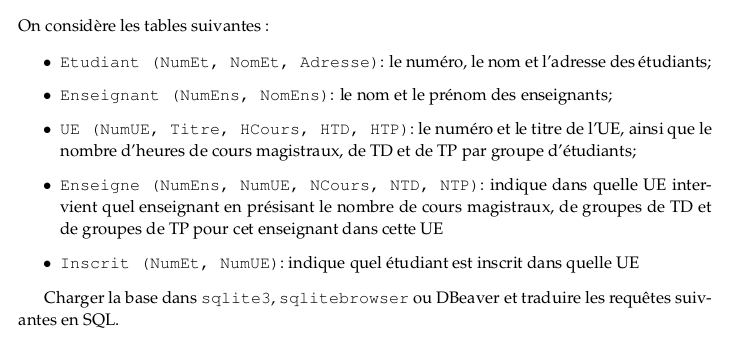
\includegraphics{base_etudiant.png}
\caption{Base étudiant}
\end{figure}

    \hypertarget{exercice-2}{%
\subsection{Exercice 2}\label{exercice-2}}

Donner les titre des UEs dans l'ordre alphabétique

    \begin{Verbatim}[commandchars=\\\{\}]
{\color{incolor}In [{\color{incolor}19}]:} \PY{o}{\PYZpc{}\PYZpc{}}\PY{k}{sql}
         
         SELECT Titre 
         FROM UE 
         ORDER BY Titre ASC;
\end{Verbatim}


    \begin{Verbatim}[commandchars=\\\{\}]
Done.

    \end{Verbatim}

\begin{Verbatim}[commandchars=\\\{\}]
{\color{outcolor}Out[{\color{outcolor}19}]:} [('Algebre',),
          ('Algorithmique',),
          ('Analyse',),
          ('Bases de donnes',),
          ('Programmation',),
          ('Reseaux',)]
\end{Verbatim}
            
    \hypertarget{exercice-3}{%
\subsection{Exercice 3:}\label{exercice-3}}

Donner le titre des UEs dont le nombre d'heures total (cours, td et cm)
par groupe est au moins 46

    \begin{Verbatim}[commandchars=\\\{\}]
{\color{incolor}In [{\color{incolor}20}]:} \PY{o}{\PYZpc{}\PYZpc{}}\PY{k}{sql}
         
         SELECT Titre 
         FROM UE 
         WHERE HCours + HTD + HTP \PYZgt{}= 46;
\end{Verbatim}


    \begin{Verbatim}[commandchars=\\\{\}]
Done.

    \end{Verbatim}

\begin{Verbatim}[commandchars=\\\{\}]
{\color{outcolor}Out[{\color{outcolor}20}]:} [('Algorithmique',), ('Bases de donnes',)]
\end{Verbatim}
            
    \hypertarget{exercice-4}{%
\subsection{Exercice 4:}\label{exercice-4}}

Donner les noms des étudiants qui ont 'Albert A.' comme enseignant.

    \begin{Verbatim}[commandchars=\\\{\}]
{\color{incolor}In [{\color{incolor}25}]:} \PY{o}{\PYZpc{}\PYZpc{}}\PY{k}{sql}
         
         SELECT DISTINCT NomEt
         FROM 
         Etudiant JOIN Inscrit
         ON Etudiant.NumET = Inscrit.NumEt
         JOIN UE
         ON Inscrit.NumUE = UE.NumUE
         JOIN Enseigne
         ON UE.NumUE = Enseigne.NumUE
         JOIN Enseignant
         ON Enseigne.NumEns = Enseignant.NumEns
         WHERE NomEns = \PYZdq{}Albert A.\PYZdq{}
         ;
\end{Verbatim}


    \begin{Verbatim}[commandchars=\\\{\}]
Done.

    \end{Verbatim}

\begin{Verbatim}[commandchars=\\\{\}]
{\color{outcolor}Out[{\color{outcolor}25}]:} [('David D.',), ('Gerald G.',), ('Jacques J.',)]
\end{Verbatim}
            
    \hypertarget{exercice-5}{%
\subsection{Exercice 5:}\label{exercice-5}}

Donner les titres des cours ayant au moins un étudiant inscrit et dont
le nombre d'heures de TD est au moins 18.

    \begin{Verbatim}[commandchars=\\\{\}]
{\color{incolor}In [{\color{incolor}34}]:} \PY{o}{\PYZpc{}\PYZpc{}}\PY{k}{sql}
         
         SELECT  Titre, HTD
         FROM 
         Etudiant JOIN Inscrit
         ON Etudiant.NumET = Inscrit.NumEt
         JOIN UE
         ON Inscrit.NumUE = UE.NumUE
         WHERE HTD \PYZgt{}= 18
         GROUP BY Titre
         ;
\end{Verbatim}


    \begin{Verbatim}[commandchars=\\\{\}]
Done.

    \end{Verbatim}

\begin{Verbatim}[commandchars=\\\{\}]
{\color{outcolor}Out[{\color{outcolor}34}]:} [('Algebre', 25.0), ('Analyse', 25.0), ('Bases de donnes', 18.0)]
\end{Verbatim}
            
    \hypertarget{exercice-6}{%
\subsection{Exercice 6:}\label{exercice-6}}

Donner les noms des enseignants qui enseignent dans la même UE que
'Albert A.' (sauf Albert A. lui-même).

    \begin{Verbatim}[commandchars=\\\{\}]
{\color{incolor}In [{\color{incolor}39}]:} \PY{o}{\PYZpc{}\PYZpc{}}\PY{k}{sql}
         
         SELECT 
             DISTINCT NomEns
             FROM 
             UE JOIN Enseigne 
             ON UE.NumUE = Enseigne.NumUE
             JOIN Enseignant 
             ON Enseigne.NumEns = Enseignant.NumEns
             WHERE NomEns != \PYZdq{}Albert A.\PYZdq{} 
             AND Titre IN (    
                     SELECT 
                         Titre
                         FROM 
                         UE JOIN Enseigne
                         ON UE.NumUE = Enseigne.NumUE
                         JOIN Enseignant
                         ON Enseigne.NumEns = Enseignant.NumEns
                         WHERE NomEns = \PYZdq{}Albert A.\PYZdq{}
                         );
\end{Verbatim}


    \begin{Verbatim}[commandchars=\\\{\}]
Done.

    \end{Verbatim}

\begin{Verbatim}[commandchars=\\\{\}]
{\color{outcolor}Out[{\color{outcolor}39}]:} [('Bertrand B.',)]
\end{Verbatim}
            
    Plutot :

    \begin{Verbatim}[commandchars=\\\{\}]
{\color{incolor}In [{\color{incolor}18}]:} \PY{o}{\PYZpc{}\PYZpc{}}\PY{k}{sql}
         
         SELECT 
             DISTINCT NomEns
             FROM Enseigne 
             JOIN Enseignant 
             ON Enseigne.NumEns = Enseignant.NumEns
             WHERE NomEns != \PYZdq{}Albert A.\PYZdq{} 
             AND NumUE IN (    
                     SELECT 
                         NumUE
                         FROM Enseigne 
                         JOIN Enseignant 
                         ON Enseigne.NumEns = Enseignant.NumEns
                         WHERE NomEns = \PYZdq{}Albert A.\PYZdq{}
                         );
\end{Verbatim}


    \begin{Verbatim}[commandchars=\\\{\}]
Done.

    \end{Verbatim}

\begin{Verbatim}[commandchars=\\\{\}]
{\color{outcolor}Out[{\color{outcolor}18}]:} [('Bertrand B.',)]
\end{Verbatim}
            
    \begin{Verbatim}[commandchars=\\\{\}]
{\color{incolor}In [{\color{incolor}17}]:} \PY{o}{\PYZpc{}\PYZpc{}}\PY{k}{sql}
         
         SELECT DISTINCT Ens2.NomEns
         FROM Enseigne AS E1
         JOIN Enseigne AS E2
         ON E2.NumUE = E1.NumUE
         JOIN Enseignant AS Ens1
         ON E1.NumEns = Ens1.NumEns
         JOIN Enseignant AS Ens2
         ON E2.NumEns = Ens2.NumEns
         WHERE Ens1.NomEns = \PYZdq{}Albert A.\PYZdq{} AND E1.NumEns \PYZlt{}\PYZgt{} E2.NumEns ;
\end{Verbatim}


    \begin{Verbatim}[commandchars=\\\{\}]
Done.

    \end{Verbatim}

\begin{Verbatim}[commandchars=\\\{\}]
{\color{outcolor}Out[{\color{outcolor}17}]:} [('Bertrand B.',)]
\end{Verbatim}
            
    \begin{Verbatim}[commandchars=\\\{\}]
{\color{incolor}In [{\color{incolor}36}]:} \PY{o}{\PYZpc{}\PYZpc{}}\PY{k}{sql}
         
         SELECT 
         NomEns, Titre
         FROM 
         UE
         JOIN Enseigne
         ON UE.NumUE = Enseigne.NumUE
         JOIN Enseignant
         ON Enseigne.NumEns = Enseignant.NumEns
         ;
\end{Verbatim}


    \begin{Verbatim}[commandchars=\\\{\}]
Done.

    \end{Verbatim}

\begin{Verbatim}[commandchars=\\\{\}]
{\color{outcolor}Out[{\color{outcolor}36}]:} [('Albert A.', 'Analyse'),
          ('Albert A.', 'Algebre'),
          ('Bertrand B.', 'Analyse'),
          ('Bertrand B.', 'Algebre'),
          ('Carine C.', 'Programmation'),
          ('Carine C.', 'Algorithmique'),
          ('Carine C.', 'Bases de donnes'),
          ('David D.', 'Programmation'),
          ('David D.', 'Algorithmique'),
          ('David D.', 'Bases de donnes'),
          ('Edgar E.', 'Programmation'),
          ('Edgar E.', 'Algorithmique'),
          ('Edgar E.', 'Bases de donnes')]
\end{Verbatim}
            
    \hypertarget{exercice-7}{%
\subsection{Exercice 7:}\label{exercice-7}}

Donner le nombre total d'heures de cours/TD/TP dispensées à
l'université. On nommera TOTAL\_HEURES ce nombre.

    \begin{Verbatim}[commandchars=\\\{\}]
{\color{incolor}In [{\color{incolor}4}]:} \PY{o}{\PYZpc{}\PYZpc{}}\PY{k}{sql}
        
        SELECT 
        SUM(HCours * NCours + HTD * NTD + HTP * NTP) AS TOTAL\PYZus{}HEURES
        FROM 
        UE
        JOIN Enseigne
        ON UE.NumUE = Enseigne.NumUE
        ;
\end{Verbatim}


    \begin{Verbatim}[commandchars=\\\{\}]
Done.

    \end{Verbatim}

\begin{Verbatim}[commandchars=\\\{\}]
{\color{outcolor}Out[{\color{outcolor}4}]:} [(436.0,)]
\end{Verbatim}
            
    \hypertarget{exercice-8}{%
\subsection{Exercice 8:}\label{exercice-8}}

Donner le nombre d'UE n'ayant pas de TP (on appellera NB\_UES l'attribut
donnant ce résultat).

    \begin{Verbatim}[commandchars=\\\{\}]
{\color{incolor}In [{\color{incolor}20}]:} \PY{o}{\PYZpc{}\PYZpc{}}\PY{k}{sql}
         
         SELECT
         COUNT(*) 
         FROM
         UE
         WHERE HTP = 0
         ;
\end{Verbatim}


    \begin{Verbatim}[commandchars=\\\{\}]
Done.

    \end{Verbatim}

\begin{Verbatim}[commandchars=\\\{\}]
{\color{outcolor}Out[{\color{outcolor}20}]:} [(2,)]
\end{Verbatim}
            
    \begin{Verbatim}[commandchars=\\\{\}]
{\color{incolor}In [{\color{incolor}19}]:} \PY{o}{\PYZpc{}\PYZpc{}}\PY{k}{sql}
         
         SELECT
         COUNT(*) 
         FROM
         (SELECT 
         UE.NumUE
         FROM 
         UE JOIN Enseigne
         ON UE.NumUE = Enseigne.NumUE
         GROUP BY UE.NumUE
         HAVING SUM(HTP * NTP) = 0
          )
         ;
\end{Verbatim}


    \begin{Verbatim}[commandchars=\\\{\}]
Done.

    \end{Verbatim}

\begin{Verbatim}[commandchars=\\\{\}]
{\color{outcolor}Out[{\color{outcolor}19}]:} [(2,)]
\end{Verbatim}
            
    Plutot la requête ci-dessous

    \begin{Verbatim}[commandchars=\\\{\}]
{\color{incolor}In [{\color{incolor}12}]:} \PY{o}{\PYZpc{}\PYZpc{}}\PY{k}{sql}
         
         SELECT 
             COUNT(*)
             FROM(
                 SELECT  Titre
                 FROM  UE
                 
                 EXCEPT
                 
                 SELECT  Titre
                 FROM UE JOIN Enseigne
                 ON UE.NumUE = Enseigne.NumUE
                 GROUP BY UE.NumUE
                 HAVING SUM(HTP * NTP) \PYZgt{} 0
             );
\end{Verbatim}


    \begin{Verbatim}[commandchars=\\\{\}]
Done.

    \end{Verbatim}

\begin{Verbatim}[commandchars=\\\{\}]
{\color{outcolor}Out[{\color{outcolor}12}]:} [(3,)]
\end{Verbatim}
            
    \hypertarget{exercice-9}{%
\subsection{Exercice 9:}\label{exercice-9}}

Donner le nombre d'étudiants qui suivent le cours d'Analyse (on
appellera NB\_ETUDIANTS l'attribut donnant ce nombre).

    \begin{Verbatim}[commandchars=\\\{\}]
{\color{incolor}In [{\color{incolor}63}]:} \PY{o}{\PYZpc{}\PYZpc{}}\PY{k}{sql}
         
         SELECT COUNT(*) AS NB\PYZus{}ETUDIANTS
         FROM 
         Etudiant JOIN Inscrit
         ON Etudiant.NumET = Inscrit.NumEt
         JOIN UE
         ON Inscrit.NumUE = UE.NumUE
         WHERE Titre = \PYZdq{}Analyse\PYZdq{}
         ;
\end{Verbatim}


    \begin{Verbatim}[commandchars=\\\{\}]
Done.

    \end{Verbatim}

\begin{Verbatim}[commandchars=\\\{\}]
{\color{outcolor}Out[{\color{outcolor}63}]:} [(3,)]
\end{Verbatim}
            
    \hypertarget{exercice-10}{%
\subsection{Exercice 10}\label{exercice-10}}

Donner la moyenne du nombre d'heures de cours, de TD et de TP par UE. On
appelera MOY\_COURS la moyenne des heures, MOY\_TD celle des TD et
MOY\_TP celle des TPs.

    \begin{Verbatim}[commandchars=\\\{\}]
{\color{incolor}In [{\color{incolor}48}]:} \PY{o}{\PYZpc{}\PYZpc{}}\PY{k}{sql}
         
         SELECT
         AVG(HCours) AS MOY\PYZus{}COURS, AVG(HTD) AS  MOY\PYZus{}TD, AVG(HTP) AS MOY\PYZus{}TP
         FROM  UE ;
\end{Verbatim}


    \begin{Verbatim}[commandchars=\\\{\}]
Done.

    \end{Verbatim}

\begin{Verbatim}[commandchars=\\\{\}]
{\color{outcolor}Out[{\color{outcolor}48}]:} [(16.5, 16.333333333333332, 8.333333333333334)]
\end{Verbatim}
            
    \hypertarget{exercice-11}{%
\subsection{Exercice 11:}\label{exercice-11}}

Donner pour chaque étudiant le nombre total d'heures qu'il suit. On
donnera dans le résultat le numéro de l'étudiant ainsi qu'un attribut
HEURES qui indiquera son nombre d'heures.

    \begin{Verbatim}[commandchars=\\\{\}]
{\color{incolor}In [{\color{incolor}15}]:} \PY{o}{\PYZpc{}\PYZpc{}}\PY{k}{sql}
         
         SELECT Etudiant.NumEt, SUM(HTP + HTD + HCours) AS HEURES
             FROM  Etudiant JOIN Inscrit
             ON Etudiant.NumET = Inscrit.NumEt
             JOIN UE
             ON Inscrit.NumUE = UE.NumUE              
             GROUP BY Etudiant.NumEt
             ORDER BY HEURES DESC
         ;
\end{Verbatim}


    \begin{Verbatim}[commandchars=\\\{\}]
Done.

    \end{Verbatim}

\begin{Verbatim}[commandchars=\\\{\}]
{\color{outcolor}Out[{\color{outcolor}15}]:} [(1117, 185.0),
          (1111, 149.0),
          (1114, 143.0),
          (1119, 135.0),
          (1112, 104.0),
          (1116, 62.0),
          (1118, 62.0),
          (1115, 50.0)]
\end{Verbatim}
            
    Plutot la requête suivante

    \begin{Verbatim}[commandchars=\\\{\}]
{\color{incolor}In [{\color{incolor}16}]:} \PY{o}{\PYZpc{}\PYZpc{}}\PY{k}{sql}
         
         SELECT NumEt, SUM(HTP + HTD + HCours) AS HEURES
             FROM  (
                     SELECT UE.NumUE, Etudiant.NumEt, HTP,  HTD, HCours  
                             Etudiant JOIN Inscrit
                             ON Etudiant.NumET = Inscrit.NumEt
                             JOIN UE
                             ON Inscrit.NumUE = UE.NumUE
                             JOIN Enseigne
                             ON UE.NumUE = Enseigne.NumUE
                         WHERE NCours+ NTD + NTP != 0
                         GROUP BY Etudiant.NumEt, UE.NumUE
                 )
             GROUP BY NumEt
             ORDER BY HEURES DESC
         ;
\end{Verbatim}


    \begin{Verbatim}[commandchars=\\\{\}]
Done.

    \end{Verbatim}

\begin{Verbatim}[commandchars=\\\{\}]
{\color{outcolor}Out[{\color{outcolor}16}]:} [(1117, 185.0),
          (1111, 149.0),
          (1114, 135.0),
          (1119, 135.0),
          (1112, 104.0),
          (1116, 54.0),
          (1118, 54.0),
          (1115, 50.0)]
\end{Verbatim}
            
    \hypertarget{exercice-12}{%
\subsection{Exercice 12:}\label{exercice-12}}

Donner les numéros des enseignants qui effectuent plus de 17 heures de
cours magistraux. Attention, ici une clause HAVING est nécessaire.

    \begin{Verbatim}[commandchars=\\\{\}]
{\color{incolor}In [{\color{incolor}49}]:} \PY{o}{\PYZpc{}\PYZpc{}}\PY{k}{sql}
         
         SELECT 
         Enseignant.NumEns,NomEns, SUM(HCours) AS HEURES\PYZus{}COURS
         FROM 
         UE
         JOIN Enseigne
         ON UE.NumUE = Enseigne.NumUE
         JOIN Enseignant
         ON Enseigne.NumEns = Enseignant.NumEns
         GROUP BY Enseignant.NumEns
         HAVING SUM(HCours * NCours) \PYZgt{} 17
         ;
\end{Verbatim}


    \begin{Verbatim}[commandchars=\\\{\}]
Done.

    \end{Verbatim}

\begin{Verbatim}[commandchars=\\\{\}]
{\color{outcolor}Out[{\color{outcolor}49}]:} [(111, 'Albert A.', 40.0),
          (112, 'Bertrand B.', 40.0),
          (114, 'David D.', 53.0),
          (115, 'Edgar E.', 53.0)]
\end{Verbatim}
            
    \begin{Verbatim}[commandchars=\\\{\}]
{\color{incolor}In [{\color{incolor}48}]:} \PY{o}{\PYZpc{}\PYZpc{}}\PY{k}{sql}
         
         SELECT 
         *
         FROM 
         UE
         JOIN Enseigne
         ON UE.NumUE = Enseigne.NumUE
         JOIN Enseignant
         ON Enseigne.NumEns = Enseignant.NumEns
         ;
\end{Verbatim}


    \begin{Verbatim}[commandchars=\\\{\}]
Done.

    \end{Verbatim}

\begin{Verbatim}[commandchars=\\\{\}]
{\color{outcolor}Out[{\color{outcolor}48}]:} [(1, 'Analyse', 20.0, 25.0, 0.0, 111, 1, 1, 1, 0, 111, 'Albert A.'),
          (2, 'Algebre', 20.0, 25.0, 0.0, 111, 2, 0, 1, 0, 111, 'Albert A.'),
          (1, 'Analyse', 20.0, 25.0, 0.0, 112, 1, 0, 1, 0, 112, 'Bertrand B.'),
          (2, 'Algebre', 20.0, 25.0, 0.0, 112, 2, 1, 1, 0, 112, 'Bertrand B.'),
          (3, 'Programmation', 15.0, 15.0, 15.0, 113, 3, 1, 1, 1, 113, 'Carine C.'),
          (4, 'Algorithmique', 20.0, 15.0, 15.0, 114, 4, 1, 1, 1, 114, 'David D.'),
          (5, 'Bases de donnes', 18.0, 18.0, 18.0, 115, 5, 1, 1, 1, 115, 'Edgar E.'),
          (4, 'Algorithmique', 20.0, 15.0, 15.0, 113, 4, 0, 0, 1, 113, 'Carine C.'),
          (5, 'Bases de donnes', 18.0, 18.0, 18.0, 113, 5, 0, 1, 1, 113, 'Carine C.'),
          (3, 'Programmation', 15.0, 15.0, 15.0, 114, 3, 0, 0, 1, 114, 'David D.'),
          (5, 'Bases de donnes', 18.0, 18.0, 18.0, 114, 5, 0, 1, 1, 114, 'David D.'),
          (3, 'Programmation', 15.0, 15.0, 15.0, 115, 3, 0, 0, 1, 115, 'Edgar E.'),
          (4, 'Algorithmique', 20.0, 15.0, 15.0, 115, 4, 0, 1, 1, 115, 'Edgar E.')]
\end{Verbatim}
            

    % Add a bibliography block to the postdoc
    
    
    
    \end{document}
